\documentclass{beamer}

\usepackage[italian]{babel}
\usepackage[utf8]{inputenc}
\usepackage[T1]{fontenc}
\usepackage{graphicx}
\usepackage{listings}
\usepackage{multicol}
\usepackage{mathtools}
\usepackage{color}
\usepackage[labelformat=empty]{caption}
\definecolor{brilliantrose}{rgb}{1.0, 0.33, 0.64}
\theoremstyle{definition}
\newtheorem{Solutions}{Solutions}

\lstset{language=java,basicstyle=\tiny\ttfamily, columns=fullflexible,
keywordstyle=\color{red}\bfseries, commentstyle=\color{blue}, frame= single,}
\renewcommand{\lstlistingname}{Codice}


\usetheme{Frankfurt}
\setbeamercovered{dynamic}
\newcommand{\nologo}{\setbeamertemplate{logo}{}} % command to set the logo to nothing


\title{Testing of chosen Design Patterns with JUnit and Mockito}
\author{\textbf{{\large Niccolò Fabbri}} \\
	\textbf{{\large Francesco Santoni}}\\
	}

\institute{Università degli Studi di Firenze\\ Master of Science in Information Engineering}
\date{24 August 2016}
\logo{
\includegraphics[width=15mm]{./LaTeX_extra/logo-unifi-1.png}}
\begin{document}

\frame{\titlepage

 Instructor: Prof. Enrico Vicario
}
\nologo
\begin{section}{Introduction}
\begin{subsection}{Introduction}
\begin{frame}
\frametitle{Introduction}
\begin{itemize}
	\item We have identified a collection of \textbf{structural} and \textbf{behavioral} \textbf{design patterns}: Class Adapter, Object Adapter, Proxy, Decorator, Composite, Observer, State, Visitor.

% ordine degli strutturali è individuato dalla "naturale" evoluzione in complessità della topologia% 
\item For each pattern we realize an implementation in Java and we develop a\textbf{ reasoned test suite} based on a realistic \textbf{fault model} and on chosen\textbf{ coverage criteria}.

\item We realize the tests through the \textit{JUnit} plug-in for Eclipse and the \textit{Mockito} framework. \textit{EclEmma} is used to provide a code coverage measure.
\end{itemize}
\end{frame}
\end{subsection}
\end{section}

\begin{section}{Design Patterns}
	\begin{subsection}{Design Patterns}
		\begin{frame}
\only<1>{			\frametitle{Class Adapter}
Adapts a pre-existent class to a new interface through inheritance.\\Through the new interface the old methods can be directly presented, modified or produce aggregated results.

\begin{figure}[!h]
	\centering
	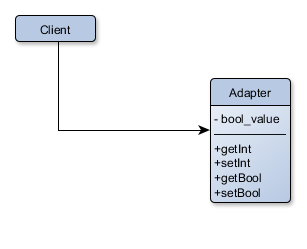
\includegraphics[width=0.74\textwidth]{./Adapter/Class/ClassDiagram.png}	
	\label{CAclassDiag}
\end{figure} 
}
	
\only<2>{
	
			\frametitle{Class Adapter - Fault Model}
Given that the pattern focuses on allowing access to legacy methods through a new interface, failures are found in the following situations:  
\begin{itemize}
	\item the adapter did not inherit from the legacy class or the new interface
	\item the adapter cannot interact with the legacy methods 
\end{itemize}
\vspace{5mm}

\begin{Solutions}

\begin{itemize}
\item test the ways in which the variable \textit{bool\_value} interacts and is modified by the methods
\end{itemize}
\end{Solutions}
	}
		\only<3>{	\frametitle{Class Adapter - Data Flow Graph}
	\begin{figure}[h]
		\centering
		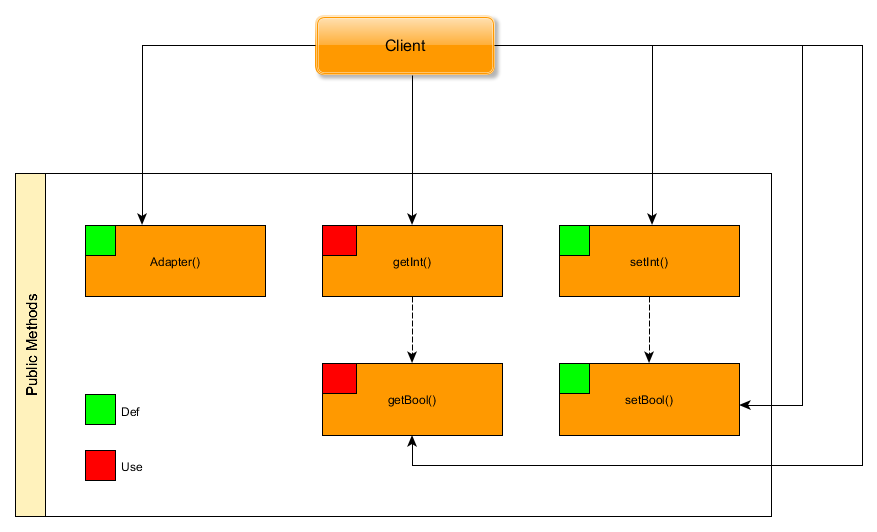
\includegraphics[width=0.74\textwidth]{./Adapter/Class/CallGraph.png}	
		\label{CAdataflow}
	\end{figure}	
\vspace{3mm}
{\footnotesize 	We generated a test suite capable of testing all the \textit{all-uses} paths:
	\begin{itemize}
		\item Adapter() getInt() 
		\item Adapter() getBool() 
		\item Adapter() setInt() getInt() 
		\item Adapter() setInt() getBool() 
		\item Adapter() setBool() getInt()
		\newline
	\end{itemize}}}

\end{frame}
\end{subsection}

	\begin{subsection}{Design Patterns}
		\begin{frame}
			
	\only<1>{		\frametitle{Object Adapter}
Adapts a pre-existent class to a new interface through class composition. Through the new interface the old methods can be directly presented, modified or produce aggregated results.

\begin{figure}[!h]
	\centering
	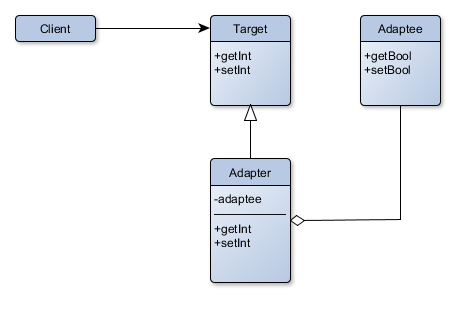
\includegraphics[width=0.74\textwidth]{./Adapter/Object/ClassDiagram.png}	
	\label{OAclassDiag}
\end{figure} 
}
\only<2>{
	\frametitle{Object Adapter - Fault Model}
	
	Given that the pattern focuses on allowing access to legacy methods through a new interface, failures are found in the following situations:  
	\begin{itemize}
		\item the adapter did not inherit from the legacy class or the new interface
		\item the adapter cannot interact with the legacy methods 
		\item the instance contained in the adapter, which inherited the adaptee class, has overrode its methods in an unforeseen way
	\end{itemize}
\vspace{3mm}
\begin{Solutions}

\begin{itemize}
	\item  test the ways in which the variable \textit{bool\_value} interacts with the methods, considering all the possible alternative implementations 
\end{itemize}
\end{Solutions}

}
	\only<3>{	\frametitle{Object Adapter - Data Flow Graph}
		\begin{figure}[h]
			\centering
			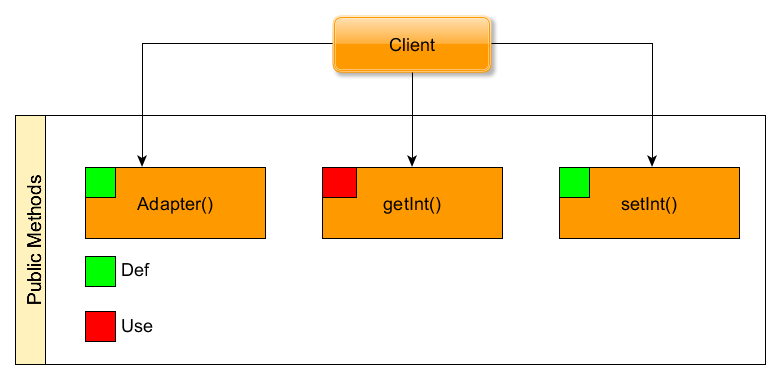
\includegraphics[width=0.75\textwidth]{./Adapter/Object/CallGraph.png}	
			\label{CAdataflow}
		\end{figure}
	{\small 	We generated a test suite capable of testing all the \textit{all-uses} paths:
		\begin{itemize}
			\item Adapter() getInt() 
			\item Adapter() setInt() getInt() 
			
		\end{itemize}
		To these are also added the topology tests:
		\begin{itemize}
			\item Adapter( Adaptee ) getInt() 
			\item Adapter( AdapteeOpposite ) getInt()
		\end{itemize}	
		}}
			
		\end{frame}
	\end{subsection}



	\begin{subsection}{Design Patterns}
		\begin{frame}
		\only{	\frametitle{Proxy}
The Proxy pattern is constituted by a class  functioning as an interface to something else, usually a complex or heavy object. It is used to access the real serving object behind the scenes, it either provides a cached result or transmits the request to the actual object.			
			\vspace{-4mm}
\begin{figure}[!h]
	\centering
	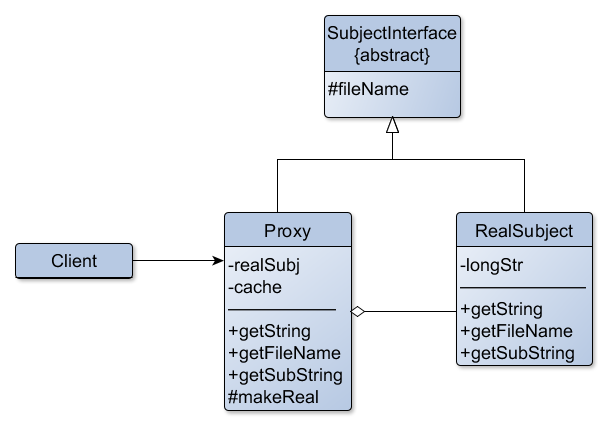
\includegraphics[width=0.72\textwidth]{./Proxy/ClassDiagram.png}
	\label{ProclassDiag}
\end{figure} }<1>
			
	
\only{		\frametitle{Proxy - Fault Model}
		
		The pattern focuses on optimizing or controlling the access to the heavy subject. We have failures in the following situations:  
		\begin{itemize}
			\item the access to the RealSubject is impeded
			\item the cached copies provided by the Proxy differ from the actual source
		\end{itemize}
		\vspace{3mm}
\begin{Solutions}
	\begin{itemize}
	\item	test the ways in which the variable \textit{realSubj} interacts and is modified by the methods \begin{itemize}
		\item[$ \rightarrow $] by slight modification of the tests we can automatically verify the cached versions validity
	\end{itemize}
	\end{itemize}
\end{Solutions}.}<2> 
		

		\only{\frametitle{Proxy - Data Flow Graph}
		\begin{figure}[!h]
		\centering
		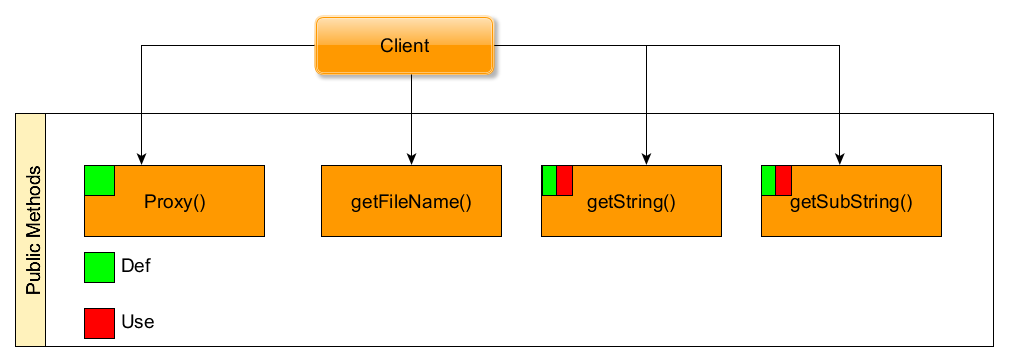
\includegraphics[width=0.85\textwidth]{./Proxy/CallGraph.png}
		
		\label{Prodataflow}
	\end{figure}
	{\footnotesize 	We generated a test suite capable of testing all the \textit{all-uses} paths:
		\begin{itemize}
			\item Proxy() getString() 
			\item Proxy() getString() getString()
			\item Proxy() getSubString()
			\item Proxy() getString() getSubString()
			\item Proxy() getSubString() getSubString()
			\item Proxy() getSubString() getString()			
		\end{itemize}}}<3> 		
		
	\end{frame}
\end{subsection}

\begin{subsection}{Design Patterns}
	\begin{frame}\only{
		\frametitle{Decorator}
		The Decorator pattern allows behavior to be added to an individual object, either statically or dynamically, without affecting the behavior of other objects from the same class.

\begin{figure}[!h]
	\centering
	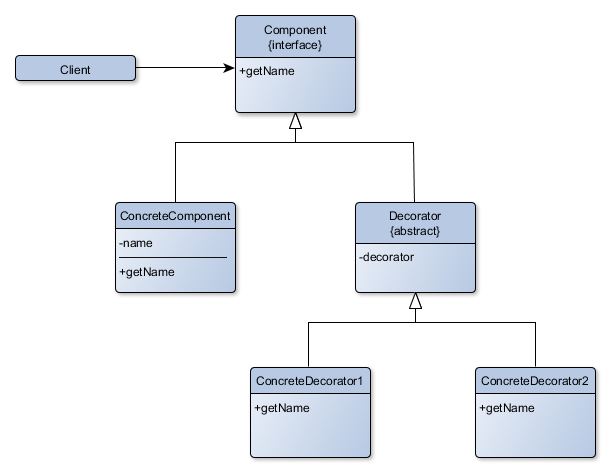
\includegraphics[width=0.75\textwidth]{./Decorator/ClassDiagram.png}	
	\label{DeclassDiag}
\end{figure} 
		}<1>
\only{		\frametitle{Decorator - Fault Model}
		
		The pattern focuses on allowing an extension of functionality in objects. Grave errors are found in the following situations:  
		\begin{itemize}
			\item the call to the \textit{operation (getName)} does not reach the Component or results in unexpected behavior
		\end{itemize}
		\vspace{3mm}
\begin{Solutions}
	\begin{itemize}
		\item test the correctness of the sequence of method calls in different hierarchies of classes
	\end{itemize}
\end{Solutions}}<2>

		

\only{		\frametitle{Decorator - Class Dependency Graph}
\begin{figure}[!h]
	\centering
	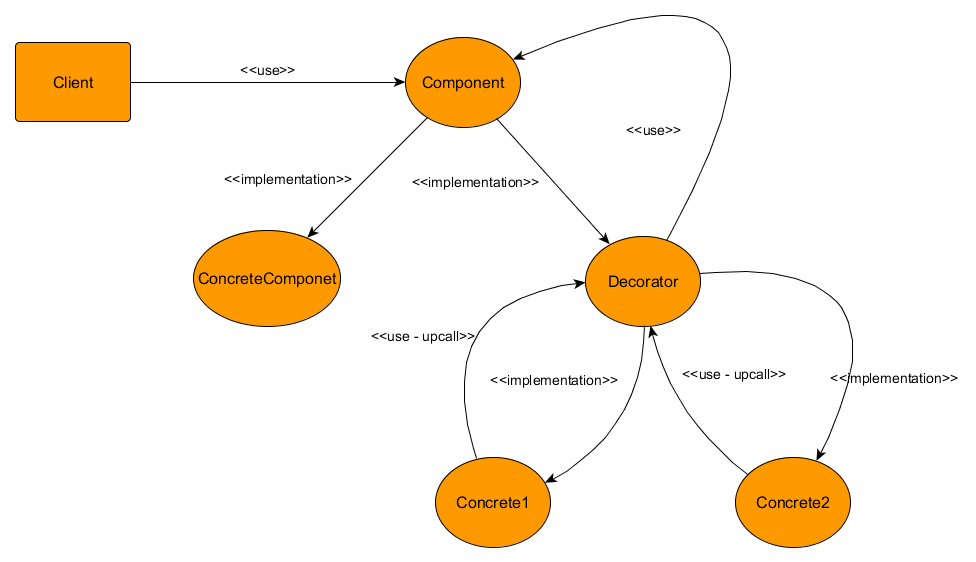
\includegraphics[width=0.95\textwidth]{./Decorator/ClassDepencyGraph.png}
	\label{Dedepengraph}
\end{figure}
{\small We decided to generate a test suite dependent on the \textit{all-edges} criterion.
We identified the 3 cases of:
\begin{itemize}
	\item ConcreteComponent
	\item Decorator ConcreteComponent
	\item Decorator Decorator ConcreteComponent
	
\end{itemize}}}<3> 		

	\end{frame}
\end{subsection}

\begin{subsection}{Design Patterns}
	\begin{frame}
		\only{\frametitle{Composite}
The Composite pattern "composes" objects into tree structures to represent part-whole hierarchies. Implementing the composite pattern lets clients treat individual objects and compositions uniformly.

\begin{figure}[!h]
	\centering
	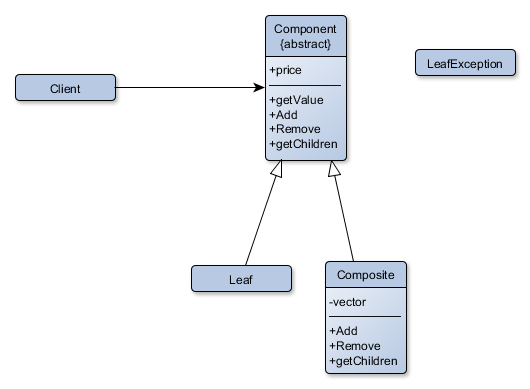
\includegraphics[width=0.8\textwidth]{./Composite/ClassDiagram.png}
	\label{CoclassDiag}
\end{figure}
		}<1>

		\only{\frametitle{Composite - Fault Model}
		
The pattern focuses on treating uniformly individual and compound objects. Grave errors are found in the following situations:  
\begin{itemize}
	\item the common \textit{operation} works differently than expected
	\item the composite-specific methods produce unexpected effects when called on a Leaf object
\end{itemize}
		\vspace{3mm}
\begin{Solutions}
	\begin{itemize}
		\item test the way \textit{operation} works under the possible hierarchies at runtime 
		\item test the way the different objects behave under calls from composite-specific methods
	\end{itemize}
\end{Solutions}}<2>


		\only{\frametitle{Composite - Data Flow Graph}

\begin{figure}[!h]
	\centering
	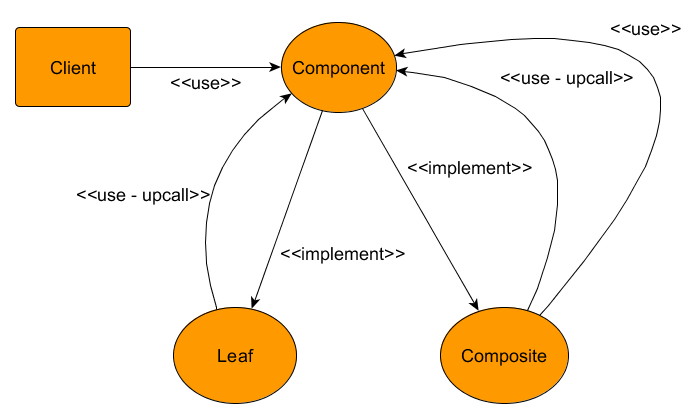
\includegraphics[width=0.8\textwidth]{./Composite/ClassDepencyGraph.png}	
	\label{Codepengraph}
\end{figure}
\vspace{-3mm}
{\footnotesize We generated a test suite capable of testing all the \textit{all-uses} paths:
\begin{itemize}
	\item Component() getChild()
	\item Component() getValue()
	\item Component() add() getChild()
	\item Component() add() getValue()
	\item Component() add() add() remove() getChild()
	\item Component() add() add() remove() getValue() 
\end{itemize}}}<3> 		

		\only{\frametitle{Composite - Class Dependency Graph}
		
		\begin{figure}[!h]
			\centering
			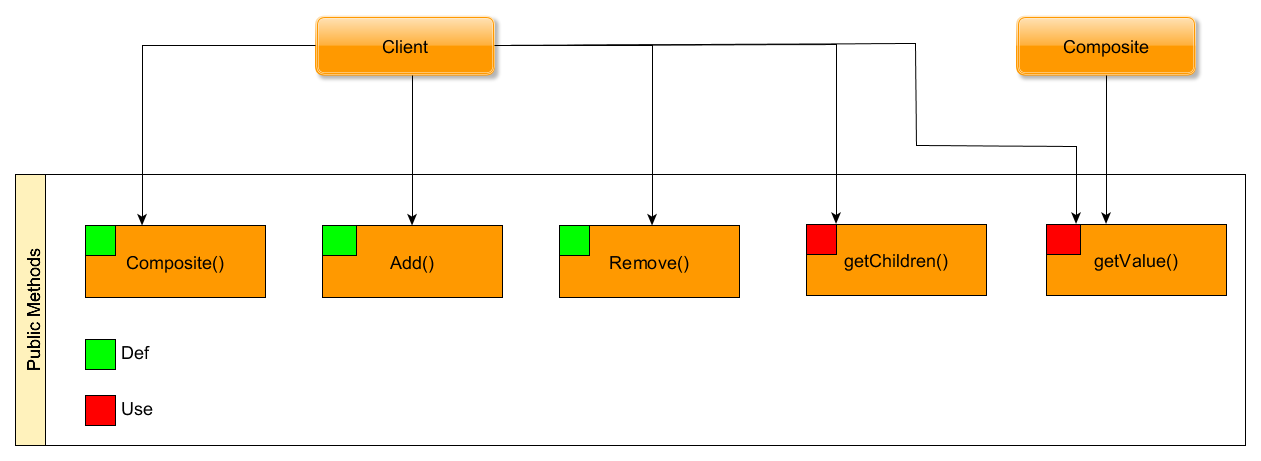
\includegraphics[width=0.87\textwidth]{./Composite/CallGraph.png}
			
			\label{Codataflow}
		\end{figure}
We identified the 3 cases of:
\begin{itemize}
	\item single Leaf
	\item Composite containing Leaf
	\item Composite containing Composite
\end{itemize}}<4>	
	\end{frame}
\end{subsection}

\begin{subsection}{Design Patterns}
	\begin{frame}
		\only{\frametitle{Observer}
		In the Observer pattern an object, called the subject, maintains a list of its dependents, called observers, and notifies them automatically of any state changes, usually by calling one of their methods.
		
\begin{figure}[!h]
	\centering
	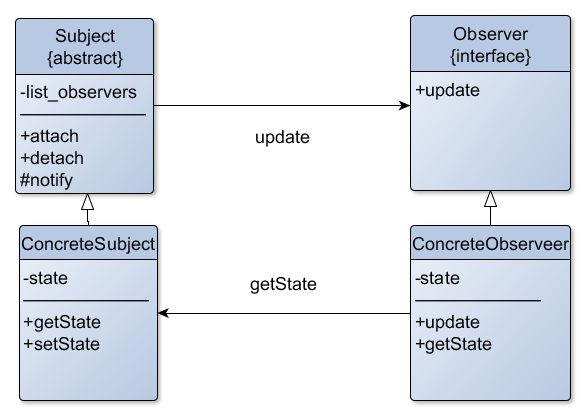
\includegraphics[width=0.74\textwidth]{./Observer/ClassDiagram.png}
	\label{ObclassDiag}
\end{figure}}<1>
		

		\only{\frametitle{Observer - Fault Model}
The pattern focuses on maintaining updated objects that expressed the interest in a specific subject. Failures are found in the following situations:  
\begin{itemize}
	\item \textit{attach} and \textit{detach} do not produce the expected results
	\item after a change of the subject state the following observers are not \textit{notified}
	\item the observer after being notified does not execute correctly the \textit{update} method
\end{itemize}
		\vspace{3mm}
\begin{Solutions}
	\begin{itemize}
			\item test the way \textit{list\_observers} is modified after an inter-class method invocation 
			\item test the way the \textit{state} of the observer is modified after a notification
	\end{itemize}
\end{Solutions}}<2>
		

		\only{\frametitle{Observer - Data Flow Graph: field \textit{list\_observer}}
\begin{figure}[!h]
	\centering
	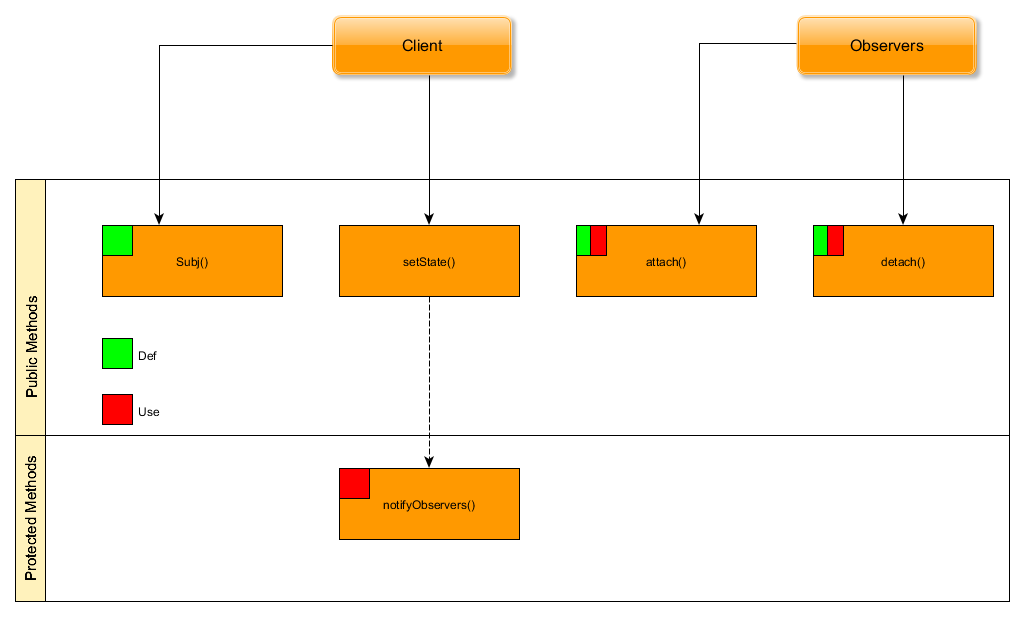
\includegraphics[width=0.8\textwidth]{./Observer/CallGraph.png}
	\label{Obdataflow1}
\end{figure} 

{\footnotesize We generated a test suite capable of testing all the \textit{all-uses} paths:
\begin{itemize}
	\item Subject() setState()[notify()]	
	\item Subject() detach() 		
	\item Subject() attach()x3 detach()x2 
	\item Subject() attach()x2 detach()x2 attach() detach() attach()
\end{itemize}		
}}<3>

		\only{\frametitle{Observer - Data Flow Graph: field \textit{state}}
		
		\begin{figure}[!h]
			\centering
			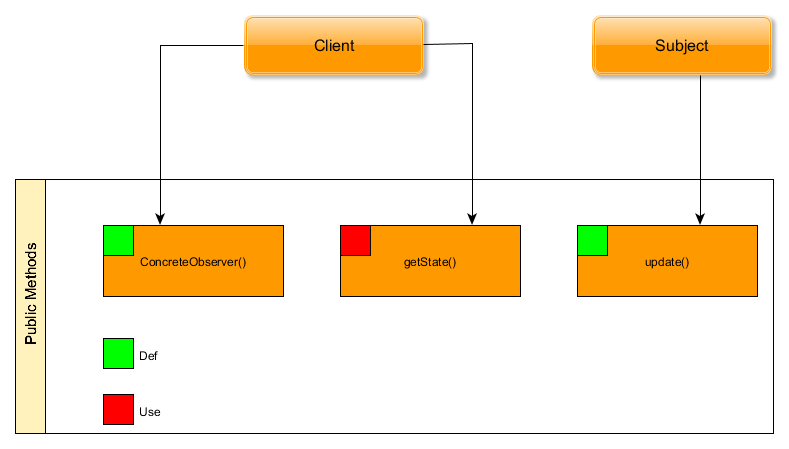
\includegraphics[width=0.8\textwidth]{./Observer/CallGraph_State.png}
			\label{Obdataflow2}
		\end{figure}
		
We generated a test suite capable of testing all the \textit{all-uses} paths:
\begin{itemize}
	\item ConcreteObserver() getState()
	\item ConcreteObserver() update() getState()
	
\end{itemize}}<4>		

	\end{frame}
\end{subsection}

\begin{subsection}{Design Patterns}
	\begin{frame}
	\only{	\frametitle{State}
		The State pattern implements a state machine by implementing each individual state as a derived class of the state pattern interface, and implementing state transitions by invoking methods defined by the pattern's superclass.
\begin{figure}[!h]
	\centering
	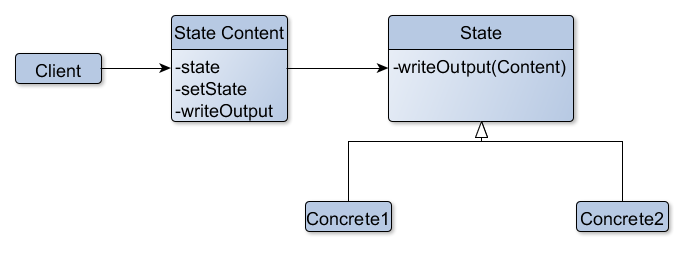
\includegraphics[width=0.8\textwidth]{./State/ClassDiagram.png}
	\label{SclassDiag}
\end{figure}}<1>
		
		\only{\frametitle{State - Fault Model}
		The pattern focuses on delegating the actual methods implementation to internal state classes. Grave errors are found in the following situations:  
		\begin{itemize}
			\item internal state changes in an erroneous manner 
			\item the internal state methods produce unexpected side effects or results
			\item the internal classes' inner state changes in an erroneous manner
		\end{itemize}
		\vspace{3mm}
		\begin{Solutions}
			\begin{itemize}
				\item test the way the \textit{state} field interacts with the StateContext methods
			\end{itemize}
		\end{Solutions}}<2>
		
		
		\only{\frametitle{State - Data Flow Graph}
\begin{figure}[!h]
	\centering
	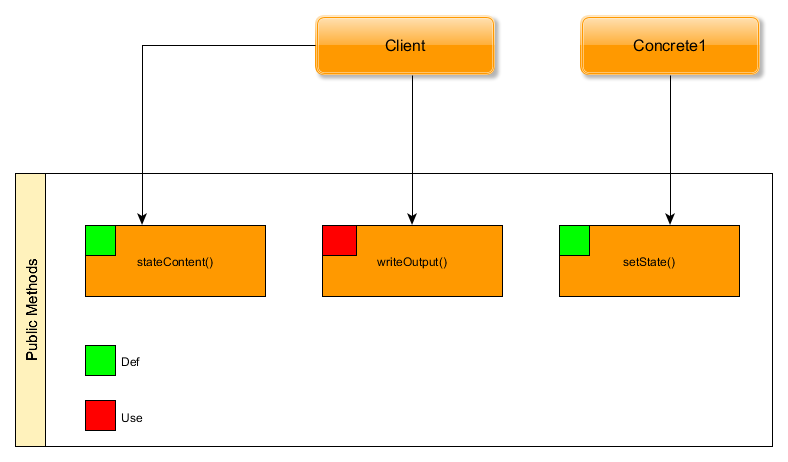
\includegraphics[width=0.8\textwidth]{./State/CallGraph.png}
	\label{Sdataflow}
\end{figure}

We generated a test suite capable of testing all the \textit{all-uses} paths:
\begin{itemize}
	\item StateContext() writeOutput() 
	\item StateContext() setState() writeOutput()
	\item StateContext() writeOutput() writeOutput()
\end{itemize}}<3>

	
	\end{frame}
\end{subsection}

\begin{subsection}{Design Patterns}
	\begin{frame}
	\only{	\frametitle{Visitor}
The Visitor pattern is a way of separating an algorithm from an object structure on which it operates. The pattern allows one to add new virtual functions to a family of classes without modifying the classes themselves.
		\vspace{-3mm}
\begin{figure}[!h]
	\centering
	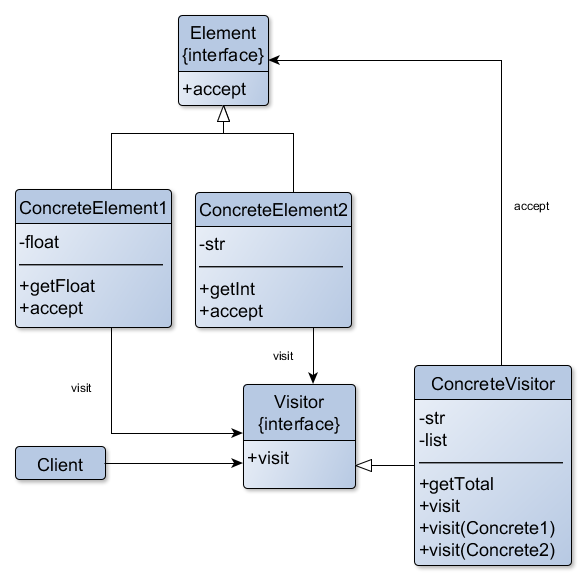
\includegraphics[width=0.96\textwidth]{./Visitor/ClassDiagram.png}
	\label{ViclassDiag}
\end{figure}}<1>
		
		\only{\frametitle{Visitor - Fault Model}
The pattern focuses on treating uniformly objects of different types while operating on them with different specializations of the same function. A failure is produced by the following situation:  
\begin{itemize}
	\item the wrong \textit{visit()} is applied to an Element
\end{itemize}
		\vspace{3mm}
\begin{Solutions}
	\begin{itemize}
		\item test the way \textit{visit} works when applied to all possible hierarchies of Element types
	\end{itemize}
\end{Solutions}}<2>
		
		\only{\frametitle{Visitor - Class Dependency Graph}
		
\begin{figure}[!h]
	\centering
	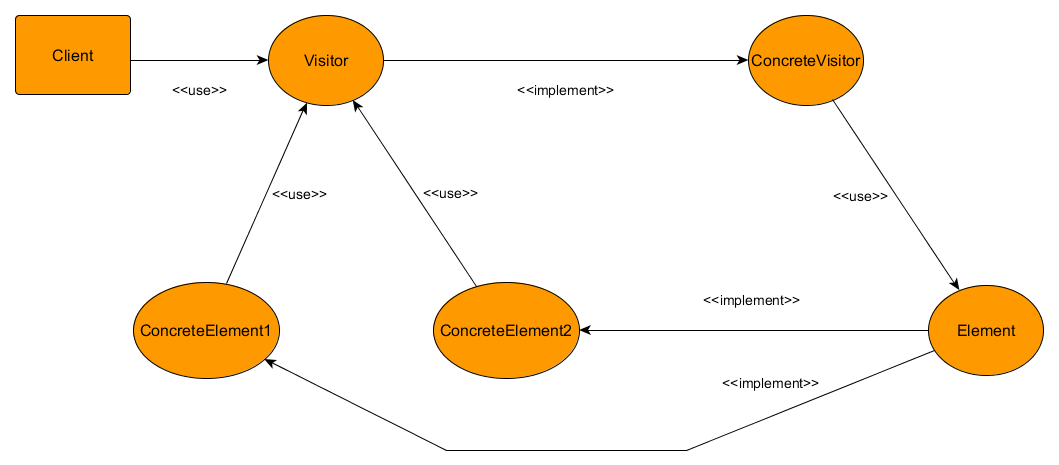
\includegraphics[width=0.84\textwidth]{./Visitor/ClassDependencyGraph.png}
	\label{Videpengraph}
\end{figure}
We identified the 2 cases of:
\begin{itemize}
	\item Visitor ConcreteVisitor Element ConcreteElement2 Visitor
	\item Visitor ConcreteVisitor Element ConcreteElement1 Visitor	
\end{itemize}}<3>
	\end{frame}
\end{subsection}
\end{section}


\begin{section}{JUnit \& Mockito}
	\begin{subsection}{JUnit \& Mockito}
		
		\begin{frame}
			
			\frametitle{JUnit}
			{\small 
				JUnit is an open source unit testing framework for the Java programming language.
				The framework allows the programmer to easily create \textit{drivers} for the tests and the ability to verify the produced outputs. 
				\begin{itemize}
					
					\item \textit{Annotation}s identify the test methods 
					\item \textit{Assertion}s tests for expected results
					
				\end{itemize}
				Main benefits of the framework are: \begin{itemize}
					\item JUnit tests can be run automatically and check their own results and provide immediate feedback without a need to manually comb through a report of test results.
					
					\item JUnit tests can be organized into test suites containing test cases and even other test suites.
					
					\item Junit shows test progress through an user-friendly bar that is green while the tests have not encountered errors and turns red when a test fails.
					
				\end{itemize}}
			\end{frame}
			\begin{frame}
				\frametitle{Mockito}
				\begin{itemize}
			\item Mockito is an open source testing framework for Java. The framework allows the creation of test double objects also called mock objects.
					
		\begin{itemize}
				\item[$ \rightarrow $] mock testing frameworks allow the faking of external dependencies so that the object being tested is isolated from external behaviors
				
				 \item[$ \rightarrow $] ensuring that objects perform the way they are expected to would require the creation of tests that actually exercise each behavior and verify that it performs as expected. \textit{Costs comparable to implementing the other classes}
				
		\end{itemize}
				\end{itemize}
				\end{frame}
				
				\begin{frame}
					\frametitle{Mockito}
									
						While utilizing the framework we identified some noteworthy details:
						\begin{itemize}
							\item in the Proxy class we utilized \textit{spy} on the very class we were testing to allow injection of other mocked classes.
							\item when using \textit{spy} the \textit{doReturn().when()} construct is to be preferred to the \textit{when().myMethod()} construct  due to the fact that the latter actually executes the function and produces side-effects before returning the designed output.
							\item returning an Answer() allows for side-effects to be produced when a mocked object's method is called. 
							\item Answer is not necessary if the side-effects are produced only on the very class under test due to the fact that one can independently produce them by simply calling the respective tested methods.
						\end{itemize}
					\end{frame}
			\end{subsection}
		\end{section}
		
		
		\begin{section}{}
			\begin{subsection}{Conclusions}
				\begin{frame}
					
					\frametitle{Conclusions}
						\begin{itemize}
						\item We identified a collection of structural and behavioral design patterns. For each pattern, we:
							{\footnotesize \begin{itemize}
								\item produced an implementation
							\end{itemize} 
							\begin{itemize}
								\item identified its main faults
							\end{itemize} 
								\begin{itemize}
									\vspace{-0.8mm}
									\item created a reasoned test suite based on the fault model and on a coverage criteria chosen pattern by pattern
								\end{itemize} }
						
						\item We realized both Unit and Integration tests through the JUnit plug - in for Eclipse and the Mockito framework.
								{\footnotesize \begin{itemize}
									\item[$ \rightarrow $] applied EclEmma to provide a code coverage measure
								\end{itemize}} 
								
						\item We identified both the untested branches and the reason for which they were not covered.
						
						\item In the end most patterns presented a full code coverage.
					\end{itemize}
					
				\end{frame}
			\end{subsection}
		\end{section}

\end{document}